\documentclass{article}

\usepackage{../../common/pnnn}

\title{Multi-layer Perceptron}
\author{Chang Lu}

\begin{document}
\maketitle

\section{Model}
Let $\mathbf{x} \in \mathbb{R}^{s \times n}$ be the inputs, where $n$ is the number of samples; and $s$ is the dimension of each feature vector. We first define a hidden layer $t$ in multi-layer perceptron (MLP):
\begin{gather}
    \mathbf{z}^{(t)} = \mathbf{w}^{(t)}\mathbf{h}^{(t - 1)} + \mathbf{b}^{(t)}, \label{eq:mlp1}\\
    \mathbf{h}^{(t)} = g^{(t)}\left(\mathbf{z}^{(t)}\right).
\end{gather}
Here, $\mathbf{h}^{(t)} \in \mathbb{R}^{d^{(t)} \times n}$ is the output of the $t$-th layer. $\mathbf{h}^{(0)} = \mathbf{x}$. $\mathbf{w}^{(t)} \in \mathbb{R}^{d^{(t)} \times d^{(t - 1)}}$ is the weight to map the output of the $(t - 1)$-th layer into the intermediate output $\mathbf{z}$. $\mathbf{b}^{(t)} \in \mathbb{R}^{d^{(t)} \times 1}$. $g^{(t)}$ is an activation function such as ReLU, sigmoid, or tanh. Typically, $g^{(t)}$ is the same among hidden layers in MLP, except the output layer. We denote the activation function in hidden layers as $g$.

In the output layer, the activation function and dimension of weights depend on specific tasks and labels. Let $C$ be the output dimension and $f$ be the activation function, the output layer is defined as follows:
\begin{gather}
    \mathbf{z}^{(T)} = \mathbf{w}^{(T)}\mathbf{h}^{(T - 1)} + \mathbf{b}^{(T)}, \\
    \hat{\mathbf{y}} = f\left(\mathbf{z}^{(T)}\right).
\end{gather}
Here, $\mathbf{w}^{(T)} \in \mathbb{R}^{C \times d^{(T - 1)}}$. Traditionally, there is an argument about counting the layers in MLP. In our project, we count one layer by the weight $w$. \figurename{~\ref{fig:mlp}} shows an example of a 2-layer MLP. It contains two hidden weight variables. We call it 2-layer MLP (input neurons, hidden neurons, and output neurons).

\begin{figure}[!ht]
    \centering
    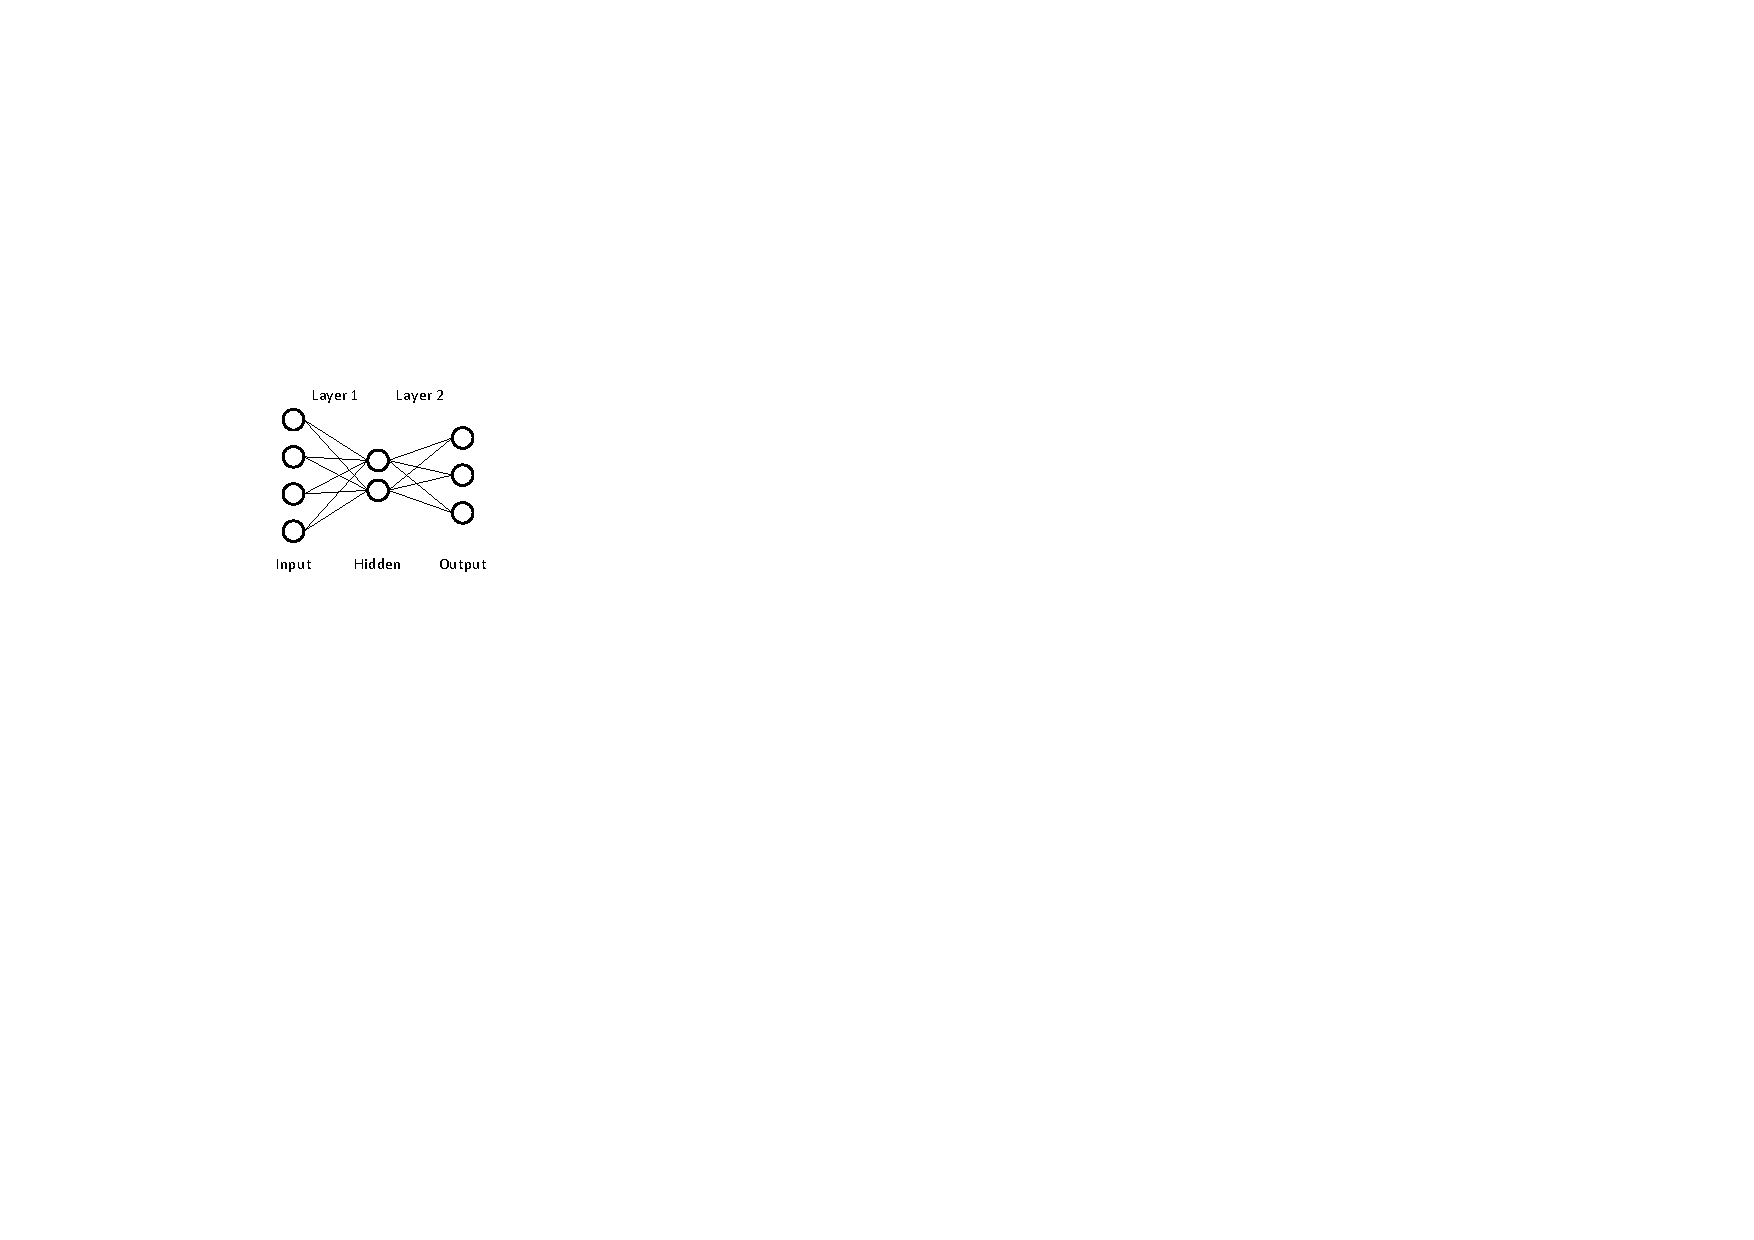
\includegraphics{figs/mlp}
    \caption{A 2-layer MLP}
    \label{fig:mlp}
\end{figure}

\section{Objective Function}
The objective function depends on various tasks. We use a multi-class classification as an example. The objective function is selected as multi-class cross-entropy loss. Let $C$ be the output dimension, i.e., number of categories and $\mathbf{y} \in \{0, 1\}^{C \times n}$ be a one-hot vector for the ground-truth, the prediction of MLP is $\hat{\mathbf{y}} \in \mathbb{R}^{C \times n}$ is a probability distribution of each entry from $\mathbf{z}^{(T)}$, calculated by a softmax activation function:
\begin{align}
    \hat{\mathbf{y}}_c = \frac{e^{\mathbf{z}^{(T)}_c}}{\sum_{k = 1}^{C}{e^{\mathbf{z}^{(T)}_k}}}. \label{eq:softmax}
\end{align}

For an input sample $\mathbf{x}_i$, the multi-class cross-entropy loss $L(\mathbf{x}_i, \mathbf{y}_i \mid \mathbf{w}^{(1)}, \dots, \mathbf{w}^{(T)})$ is:
\begin{align}
    L(\mathbf{x}_i, \mathbf{y}_i \mid \mathbf{w}^{(1)}, \dots, \mathbf{w}^{(T)}) &= -\sum_{c = 1}^{C}{\mathbf{y}_{c, i}\log{\hat{\mathbf{y}}_{c, i}}} \\
    &= -\sum_{c = 1}^{C}{\mathbf{y}_{c, i}\left(\mathbf{z}^{(T)}_{c, i} - \log{\sum_{k = 1}^{C}{e^{\mathbf{z}^{(T)}_{i, k}}}}\right)} \notag \\
    &= \log{\sum_{c = 1}^{C}{e^{\mathbf{z}^{(T)}_{c, i}}}} - \sum_{c = 1}^{C}{\mathbf{y}_{c, i}\mathbf{z}^{(T)}_{c, i}}. \label{eq:logsumexp}
\end{align}

For all input samples $\mathbf{x}$, the total loss is an average of the losses for all samples:
\begin{align}
    L(\mathbf{x}, \mathbf{y} \mid \mathbf{w}^{(1)}, \dots, \mathbf{w}^{(T)}) &= -\frac{1}{n}\sum_{i = 1}^{n}{\sum_{c = 1}^{C}{\mathbf{y}_{c, i}\log{\hat{\mathbf{y}}_{c, i}}}} \notag \\
    &= \frac{1}{n}\sum_{i = 1}^{n}{\left(\log{\sum_{c = 1}^{C}{e^{\mathbf{z}^{(T)}_{c, i}}}} - \sum_{c = 1}^{C}{\mathbf{y}_{c, i}\mathbf{z}^{(T)}_{c, i}}\right)}.
\end{align}

\subsection{A Trick for Stable Softmax and Log-Sum-Exp}
When calculating $e^x$ for softmax function in Equation~\eqref{eq:softmax} and Equation~\eqref{eq:logsumexp}, $x$ can be large so that there may be a numerical problem. To alleviate this problem, we can take advantage a property of softmax:
\begin{align}
    \text{softmax}(x_c \mid x_1, \dots, x_C) &= \frac{e^{x_c}}{\sum_{k = 1}^{C}{e^{x_c}}} = \frac{e^{-\lambda} \cdot e^{x_c}}{e^{-\lambda} \cdot \sum_{k = 1}^{C}{e^{x_c}}} = \frac{e^{x_c - \lambda}}{\sum_{k = 1}^{C}{e^{x_c - \lambda}}} \notag \\
    &= \text{softmax}(x_c - \lambda \mid x_1 - \lambda, \dots, x_C - \lambda).
\end{align}

Similarly, we can get
\begin{align}
    \log{\sum_{c = 1}^{C}{e^{x_c}}} &= \log{\left(e^{\lambda} \cdot e^{-\lambda} \cdot \sum_{c = 1}^{C}{e^{x_c}}\right)} = \lambda + \log{\sum_{c = 1}^{C}{e^{x_c - \lambda}}}.
\end{align}
Let $\lambda = \max{\{x_1, x_2, \dots, x_C\}}$, for $\forall c \ge 1$ and $c \le C$, we have $x_c - \lambda \le 0 \Rightarrow e^{x_c - \lambda} \le 1$. In this way, the softmax and log-sum-exp operations can be numerically stable.

\section{Back-propagation}
We use the multi-class classification for predictions and ReLU activation for hidden layers. The trainable variables are $\mathbf{w}^{(1)}, \dots, \mathbf{w}^{(T)}$ and $\mathbf{b}^{(1)}, \dots, \mathbf{b}^{(T)}$. We need to calculate gradients for all of these variables. For $\mathbf{w}^{(t)}$, we need to apply the chain rule:
\begin{align}
    \pb{L}{\mathbf{w}^{(t)}} = \pb{L}{\mathbf{z}^{(t)}}\pb{\mathbf{z}^{(t)}}{\mathbf{w}^{(t)}} \in \mathbb{R}^{d^{(t - 1)} \times d^{(t)}}. \notag
\end{align}
For the first term, it is not easy to directly get the gradient of $\mathbf{z}^{(t)}$. For the second term, it is a matrix-by-matrix derivative, we cannot directly calculate either. Therefore, we first consider the loss of one sample: $L_i = L(\mathbf{x}_i, \mathbf{y}_i)$. Then we seek to pass gradients from the $(t + 1)$-th layer w.r.t. the $k$-th row of $\mathbf{w}^{t}$. Let
\begin{align}
    \phi(t, i) &= \pb{L_{i}}{\mathbf{z}^{(t)}_{:i}} \in \mathbb{R}^{1 \times d^{(t)}}, \notag \\
    \psi(t, i, k) &= \pb{L_{i}}{{\mathbf{w}^{(t)}_{k:}}^\top} \in \mathbb{R}^{1 \times d^{(t - 1)}}, \notag
\end{align}
we have
\begin{align}
    \phi(t, i) &= \underbrace{\phi(t + 1, i)}_{1 \times d^{(t + 1)}} \underbrace{\pb{\mathbf{z}^{(t + 1)}_{:i}}{\mathbf{z}^{(t)}_{:i}}}_{d^{(t + 1)} \times d^{(t)}}, \notag \\
    \psi(t, i, k) &= \underbrace{\phi(t, i)}_{1 \times d^{(t)}}\underbrace{\pb{\mathbf{z}^{(t)}_{:i}}{{\mathbf{w}^{(t)}_{k:}}^\top}}_{d^{(t)} \times d^{(t - 1)}}. \notag
\end{align}
In this way, we only need to calculate $\phi(T, i), \pb{\mathbf{z}^{(t + 1)}_{:i}}{\mathbf{z}^{(t)}_{:i}}$, and $\pb{\mathbf{z}^{(t)}_{:i}}{{\mathbf{w}^{(t)}_{k:}}^\top}$, which is easier and intuitive. Then a recursive way can be applied to calculate each $\mathbf{w}^{(t)}$.
\begin{align}
    \phi(T, i) &= {\pa{\mathbf{z}^{(T)}_{:i}}\left(\log{\sum_{c = 1}^{C}{e^{\mathbf{z}^{(T)}_{c, i}}}} - \sum_{c = 1}^{C}{\mathbf{y}_{c, i}\mathbf{z}^{(T)}_{c, i}}\right)} \notag \\
    &= {\pa{\mathbf{z}^{(T)}_{:i}}\log{\sum_{c = 1}^{C}{e^{\mathbf{z}^{(T)}_{c, i}}}}} - {\pa{\mathbf{z}^{(T)}_{:i}}\sum_{c = 1}^{C}{\mathbf{y}_{c, i}\mathbf{z}^{(T)}_{c, i}}} \notag \\
    &= \frac{1}{\sum_{c = 1}^{C}{e^{\mathbf{z}^{(T)}_{c, i}}}} \cdot \pa{\mathbf{z}^{(T)}_{:i}}\left(\sum_{c = 1}^{C}{e^{\mathbf{z}^{(T)}_{c, i}}}\right) - {\pa{\mathbf{z}^{(T)}_{:i}}\left(\sum_{c = 1}^{C}{\mathbf{y}_{c, i}\mathbf{z}^{(T)}_{c, i}}\right)} \notag \\
    &= \frac{1}{\sum_{c = 1}^{C}{e^{\mathbf{z}^{(T)}_{c, i}}}} \cdot {e^{\mathbf{z}^{(T)}_{:i}}}^\top - \mathbf{y}_{:i}^\top \notag \\
    &= \left(\hat{\mathbf{y}}_{:i} - \mathbf{y}_{:i}\right)^\top. \notag \\
    \pb{\mathbf{z}^{(t + 1)}_{:i}}{\mathbf{z}^{(t)}_{:i}} &= \pb{\mathbf{z}^{(t + 1)}_{:i}}{\mathbf{h}^{(t)}_{:i}}\pb{\mathbf{h}^{(t)}_{:i}}{\mathbf{z}^{(t)}_{:i}} = \mathbf{w}^{(t + 1)}\text{Diag}\left(\text{ReLU}'\left(\mathbf{z}^{(t)}_{:i}\right)\right). \notag
\end{align}
Here, ReLU$'(\cdot)$ is the derivative of ReLU function. We will give its formal definition later. Diag$(\cdot)$ is a diagnal matrix of which the main diagnal is the given input vector. Therefore, we can derive
\begin{align}
    \phi(t, i) &= \phi(t + 1, i)\pb{\mathbf{z}^{(t + 1)}_{:i}}{\mathbf{z}^{(t)}_{:i}} \notag \\
    &= \phi(t + 1, i)\mathbf{w}^{(t + 1)}\text{Diag}\left(\text{ReLU}'\left(\mathbf{z}^{(t)}_{:i}\right)\right) \notag \\
    &= \left(\phi(t + 1, i)\mathbf{w}^{(t + 1)}\right) \odot \text{ReLU}'\left(\mathbf{z}^{(t)}_{:i}\right)^\top \notag
\end{align}
Here, $\odot$ denotes element-wise product for two column/row vectors. For $\pb{\mathbf{z}^{(t)}_{:i}}{{\mathbf{w}^{(t)}_{k:}}^\top}$, it is a $d^{(t)} \times d^{(t)}$ matrix. We denote it as $\mathbf{X}$.
\begin{align}
    \pb{\mathbf{z}^{(t)}_{:i}}{{\mathbf{w}^{(t)}_{k:}}^\top} &= \mathbf{X}, \notag
\end{align}
\begin{align}
    \text{where}~\mathbf{X}_{j:} &= \begin{cases}
        {\mathbf{h}^{(t - 1)}_{:i}}^\top &~\text{if}~j = k, \\
        \mathbf{0} &~\text{otherwise}.
    \end{cases} \notag
\end{align}
Therefore, we can derive
\begin{align}
    \psi(t, i, k) &= \phi(t, i)\mathbf{X} = \phi(t, i)_m \cdot \mathbf{X}_{k:} = \phi(t, i)_m \cdot {\mathbf{h}^{(t - 1)}_{:i}}^\top. \notag
\end{align}
Since $\psi(t, i, k)$ is for the $k$-th row of $\mathbf{w}^{(t)}$, for the complete $\mathbf{w}^{(t)}$, we have
\begin{align}
    \pb{L_{i}}{{\mathbf{w}^{(t)}}} = \psi(t, i) = \left[\psi(t, i, 1)^\top, \psi(t, i, 2)^\top, \dots, \psi(t, i, d^{(t)})^\top\right] = \mathbf{h}^{(t - 1)}_{:i}\phi(t, i). \notag
\end{align}

Here, we have already got the gradient for one sample. For all samples, we need to rewrite the $\phi(t, i)$ and $\psi(t, i)$ to a matrix form $\phi(t)$ and $\psi(t)$:
\begin{align}
    \pb{L}{\mathbf{z}^{(T)}} &= \phi(T) = \left(\hat{\mathbf{y}} - \mathbf{y}\right)^\top \in \mathbb{R}^{n \times C}, \label{eq:phiT} \\
    \pb{L}{\mathbf{z}^{(t)}} &= \phi(t) = \left(\phi(t + 1)\mathbf{w}^{(t + 1)}\right) \odot \text{ReLU}'\left(\mathbf{z}^{(t)}\right)^\top \label{eq:phit} \in \mathbb{R}^{n \times d^{(t)}}, \\
    \pb{L}{\mathbf{w}^{(t)}} &= \psi(t) = \frac{1}{n}\sum_{i = 1}^{n}{\psi(t, i)} = \frac{1}{n}\mathbf{h}^{(t - 1)}\phi(t) \in \mathbb{R}^{d^{(t - 1)} \times d^{(t)}}. \label{eq:psit}
\end{align}
Similarly, the gradient of $\mathbf{b}^{(t)}$ can be calculated as:
\begin{align}
    \pb{L}{\mathbf{b}^{(t)}} = \frac{1}{n}\phi(t) \in \mathbb{R}^{1 \times d^{(t)}}. \label{eq:bt}
\end{align}
Equations~\eqref{eq:phiT}-\eqref{eq:bt} are the final gradients for MLP. For the dimension of matrix derivative, please refer to \href{https://en.wikipedia.org/wiki/Matrix_calculus}{Matrix Calculus at Wikipedia}.

\paragraph{Recap.} We may notice that the gradients of the output layer ($t = T$) of MLP is similar to the logistic regression. In fact, the binary classification is a special form of multi-class classification, and logistic regression can be regraded as a single-layer MLP. In practice, the label of binary classification is usually 0 or 1, while the label of multi-class classification is a one-hot vector. This is the reason why we distinguish binary classification from multi-class classification.

After getting the gredients of weights and bias in MLP, there is still a derivative of ReLU activation function to be solved. The ReLU function is defined as follows:
\begin{align}
    \text{ReLU}\left(x\right) = \begin{cases}
        0 &~\text{if}~x < 0, \\
        x &~\text{otherwise},
    \end{cases} = \max\{0, x\}.
\end{align}
It is a convex function that is sub-differential when $x \ne 0$. However, it is undifferentiable at $x = 0$. Therefore, we use subgradient of ReLU and set the gradient as 0 at $x = 0$:
\begin{align}
    \text{ReLU}'\left(x\right) = \begin{cases}
        0 &~\text{if}~x \le 0, \\
        1 &~\text{otherwise}.
    \end{cases}
\end{align}

\end{document}